\documentclass[12pt]{article}
\usepackage{graphicx}
%
% Title[Enter title of the experiment here]
\title{EE230: Analog Circuits Lab\\ Lab No.}
% Author[Enter details of author here]
\author{Name of student,Roll. no.}

% begin the document.
\begin{document}

% make a title page.[this creates title page]
\maketitle

\textbf{ ** All experiment reports may not contain all fields in this format,This document is just for your reference**} 

\section{Title of the experiment 1}
**For each experiment a new section has to be created**
\subsection{Aim of the experiment}

In your own words, describe the aim of the experiment.


\subsection{Design}

In this section, explain your design strategy for the experiment.Mention all the design steps you follow for each part of the experiment.An equation based analysis, with supporting circuit diagrams is expected. \textbf{Circuit diagrams must be made in Xcircuit}.
 
 \begin{equation}
     v_{o1}-v_{o2}
     \newline
     = -g_mR_D(v_{in1}-v_{in2})
 \end{equation}     
 
 \begin{equation}
     a=b+c
 \end{equation}     

 %equations are to inserted in this manner.
\begin{figure}[h!]
\centering
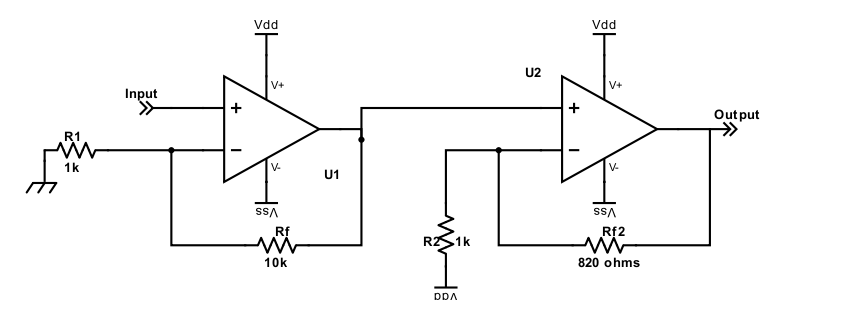
\includegraphics[scale = 0.4]{hall_amp.png}
\end{figure}

\textbf{(copy-paste from handout will be counted as plagiarism).} 

%\textbf{this command prints text inside it in bold style}


\subsection{Simulation results}%[One more section] 
**\textbf{Add this section if mentioned in the handout}**
\subsubsection{Circuit Schematics}
Enter the circuit schematics drawn on the LTSpice.
\begin{figure}[h!]
\centering
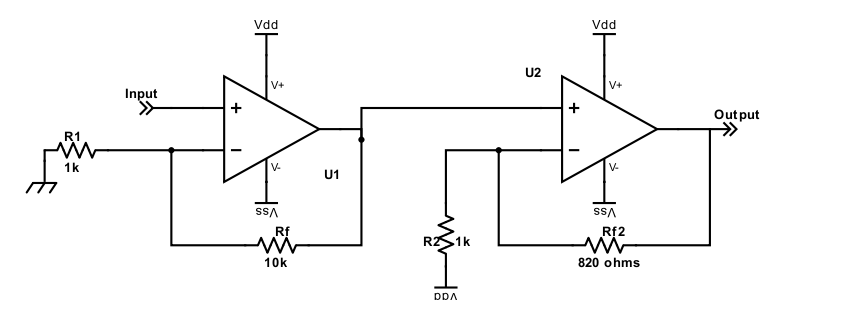
\includegraphics[scale = 0.4]{hall_amp.png}
\end{figure}

\subsubsection{Simulation results}

Enter your simulation plots, together with text explaining the plots. All figures must have legible fonts, and a caption that makes sense.


\begin{figure}[h!]

\centering
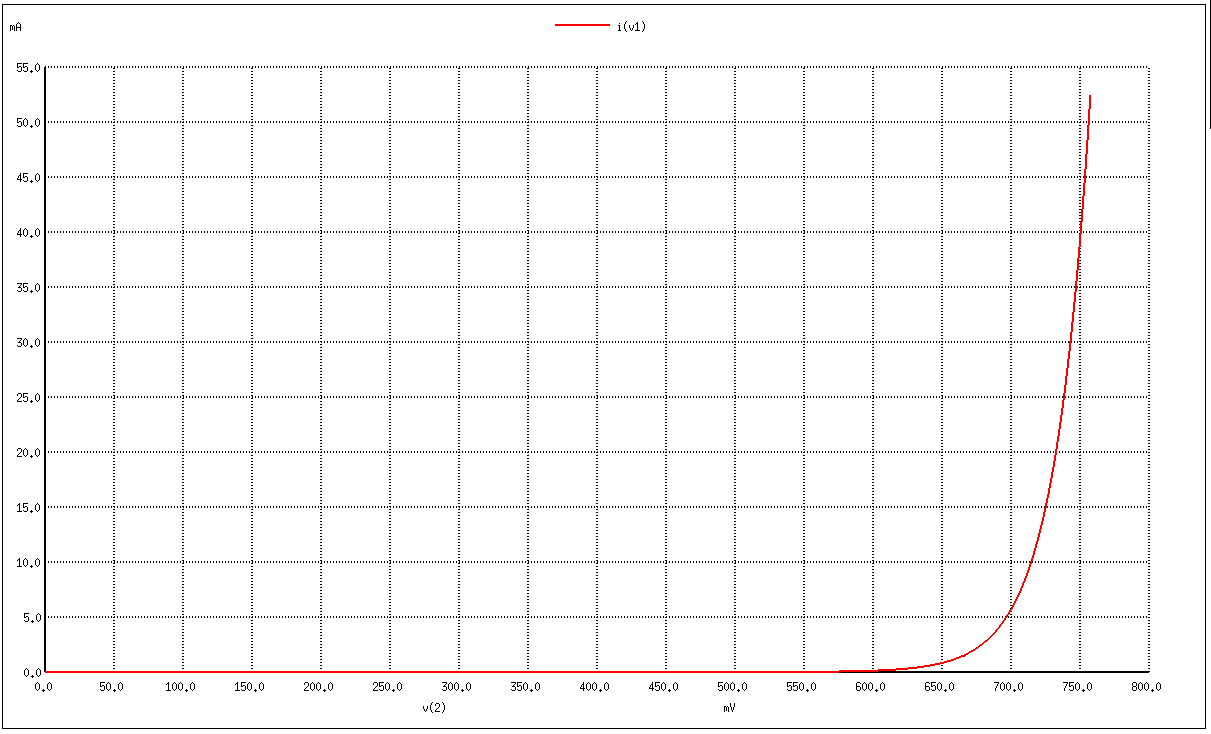
\includegraphics[scale = 0.2]{normaldiode.png}
\end{figure}
  \newpage


\subsection{Experimental results}

Results of the experiment should be added here.Mention what component values you used with appropriate circuit diagram, and what your measured and theoretical values were. \\

**Create subsections similar to the sections created in handout.**
\begin{table}[!hbt]
		% Center the table
		\begin{center}
		\caption{Table Caption}
		\begin{tabular}{|c|c|c|c|}
			% To create a horizontal line, type \hline
			\hline
			% To end a column type &
			% For a linebreak type \\
			Sr. No. & column1 & column2 & column3\\
			\hline
			row1 &  &  & \\
			\hline
			row2 &  &  & \\
			\hline
            
		\end{tabular}
		\end{center}
\end{table}

\subsection{Conclusion and Inference}
Conclusion and Inference of the experiment should be added here.


\subsection{Experiment completion status}
In this part, mention which sections you completed in lab and which you couldn't,also give suitable explanation stating why you couldn't complete it.

\newpage
\section{Title of the experiment 2}
**Each experiment should start on new page**
\subsection{Aim of the experiment}
\subsection{Design}
\subsection{Simulation results}
\subsection{Experimental results}
\subsection{Conclusion and Inference}
\subsection{Experiment completion status}

** Add more experiments section (on new page) if applicable**

\end{document}
